\Chapter{Testek optimalizálása}

Érdemes megnézni, hogy egyes testeknél hogyan tudunk konvergálni különböző eloszlásokhoz.
Ehhez a \ref{sect:ratiomodification} szakaszban bemutatott heurisztikát fogjuk használni.
Addig módosítjuk a testeket, amíg az oldallapokhoz tartozó relatív hiba az általunk megadott küszöbérték alá nem esik.
Ezt a küszöböt $\chi^2$-re nézve az alábbi összefüggéssel írhatjuk fel:
\[
\chi^2 < N \cdot error^2,
\]
ahol $N$ a dobássorozat száma és $error$ az általunk megadott hibaküszöb.
Ezt a küszöböt tudnánk igazítani ahhoz is, hogy a módosított testet milyen szignifikancia szinten szeretnénk elfogadni.
Testenként változó, hogy egy adott $\alpha$ szignifikancia szinthez tartozó  $\chi^2$ érték maximum mennyi lehet, és annak nagysága nagyban függ a dobássorozatok méretétől, ezért a fent leírt képlettel fogjuk számolni a hibaküszöböt.

A fejezet további részében az optimalizálások fognak történni.
Mindegyik mérésről lesz egy leírás, hogy miért azt az eloszlást választottuk, milyen eredményre számítunk.
A testek és a várt eloszlás leírása után fognak szerepelni a futásnál használt paraméterek és a konvergencia görbe.
Végül az egyéb tapasztalatok jönnek, hogy mennyire hasonlít a test az általunk elképzelt alakzatra.

\Section{Tetraéder}

Az alap tetraéder, amit módosítani fogunk 50 egység hosszú oldallapokkal rendelkezik.
Hogy a módosított alakzatokat $\alpha = 0.05$ szignifikancia szinten el tudjuk fogadni a $\chi^2 < 7.815$ feltételnek teljesülnie kell.

A módosító algoritmusok leírásánál ezen a testen végeztünk teszteket, és mindig a [0.1, 0.2, 0.3, 0.4] eloszlást közelítettük.
Azért ezeket az értékeket választottuk, mert itt egyértelműen látszódik az egyes oldallapok közötti különbség, valamint könnyen meg tudjuk határozni ránézésre hogy a mért frekvenciák mennyire térnek el az elvárt értékektől.

\begin{python}
from jelly.py import Tetrahedron
err = 0.05
N = 1000
threshold = n * err**2
tetrahedron = Tetrahedron()
t1 = tetrahedron.estimateBodyFace2([0.1,0.2,0.3,0.4],1,threshold,N)[0]
\end{python}

\begin{figure}[h!]
	\centering
	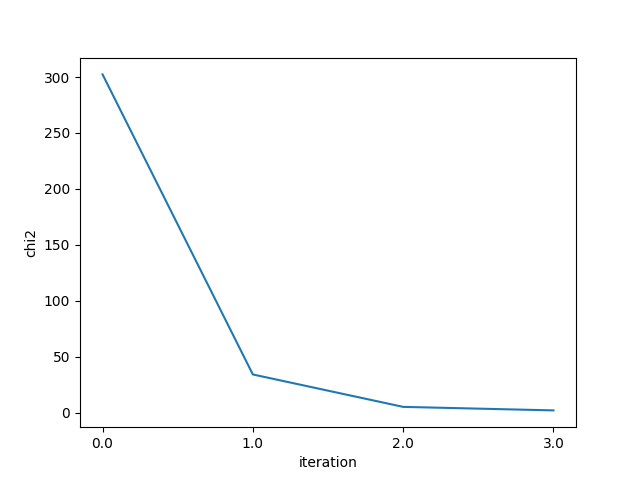
\includegraphics[scale=0.7]{images/tetrahedron_01.png}
	\caption{Az első tetraéder konvergencia görbéje.}
	\label{fig:tetra01}
\end{figure}
%end chi2 = 1.9608333333333332

A \ref{fig:tetra01} grafikonon látható a konvergenciája a testnek az említett eloszláshoz.
Látható hogy a választott teszt eloszlás nem csak vizsgálat szempontjából előnyös, hanem könnyen elérhető.

A következő test a \textit{Dark Souls: The Board Game}-ben használt narancssárga dobókocka közelítése.
A kocka oldallapjain található értékek a következőek: 1 darab egyes, 2 darab kettes, 2 darab hármas és 1 darab négyes.
Mivel csak négy érték fordul elő, ezért lehet a testet egy tetraéderrel közelíteni, aminek várhatóan kettő oldallapja nagyobb, kettő oldallapja pedig kisebb lesz.

\begin{python}
from jelly.py import Tetrahedron
err = 0.05
N = 1000
threshold = n * err**2
tetrahedron = Tetrahedron()
t2 = tetrahedron.estimateBodyFace2([1/6,1/3,1/3,1/6],1,threshold,N)[0]
\end{python}

\begin{figure}[h!]
	\centering
	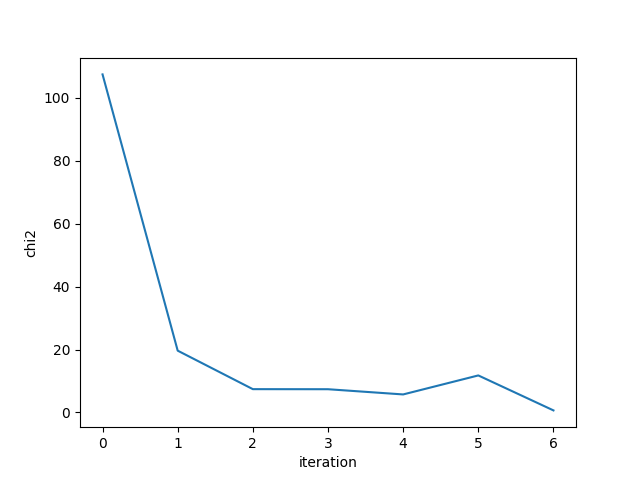
\includegraphics[scale=0.7]{images/tetrahedron_02.png}
	\caption{Az második tetraéder konvergencia görbéje.}
	\label{fig:tetra02}
\end{figure}
%end chi2 = 3.689

A \ref{fig:tetra02} grafikonon látható, hogy a választott eloszlás elérése nem olyan triviális.
Az algoritmus követ el hibákat, amelyek a test alakja miatt nem okoznak látványos változást a görbén.

A kapott testen oldallapjai egyenlő szárú háromszögekhez hasonlítanak, amelyeknek az alapjuk más hosszúságú.
Felismerhető, hogy kis hibával különböznek az egyforma lappárok, valamint az alap feltételezésünk, hogy a ritkább előfordulású oldallapok területe ki lesz beigazolódott.

\newpage

\Section{Dupla tetraéder}

A dupla tetraéder a sima változatához hasonlóan 50 egység hosszú oldalélekkel fog rendelkezni.
A $\chi^2$ próbánál hogy $\alpha = 0.05$ szignifikancia szinten el tudjuk fogadni a módosítást a $\chi^2$-nek kisebbnek kell lennie mint $11.07$.


A tetraéderhez hasonlóan egy egyszerűbbnek tűnő eloszlással fogunk kipróbálni.
Az eloszlás: [1/12, 2/12, 3/12, 3/12, 2/12, 1/12].

\begin{python}
from jelly.py import DoubleTetrahedron
err = 0.05
N = 1000
threshold = n * err**2
doubletetrahedron = DoubleTetrahedron()
dt1 = doubletetrahedron.estimateBodyFace2(
      [1/12, 2/12, 3/12, 3/12, 2/12, 1/12],
      1, threshold, N)[0]
\end{python}

\begin{figure}[h!]
	\centering
	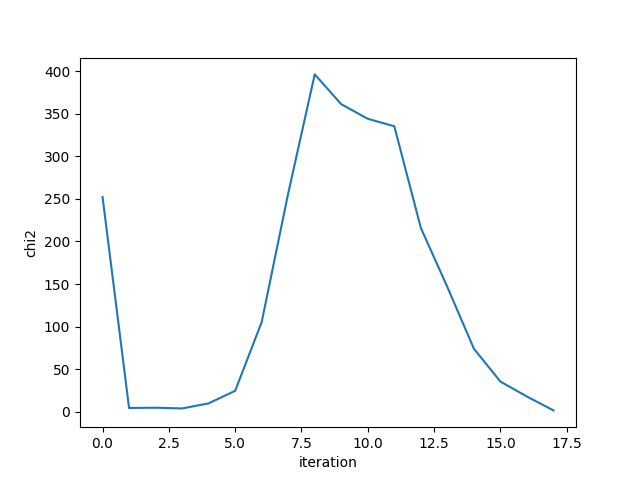
\includegraphics[scale=0.7]{images/doubletetrahedron_01.png}
	\caption{Az első dupla tetraéder konvergencia görbéje.}
	\label{fig:doubletetra01}
\end{figure}
%after test chi2 = 1.9919999999999995

A \ref{fig:doubletetra01} grafikonon látható, hogy az 5. iterációtól kezdve elkezdett az algoritmus egyre rosszabb értékeket kapni, és csak utána tudott a megfelelő értékhez konvergálni.
Ez amiatt történt, hogy a $\chi^2$ érték nagyon közel került a küszöbértékhez, és a következő iterációkban lévő fokozatos romlás a $\lambda$ értéknek köszönhető.
Ilyen esetekre számítottunk amikor a \ref{sect:ratiomodification} szakaszban a $\lambda$ értéket akartuk meghatározni.

A következő módosításnál a [2/15, 2/15, 2/15, 2/15, 2/15, 1/3] eloszlást szeretnénk elérni.
Arra számítunk, hogy egy olyan "cinklet" testet kapunk, amelyen az egyik oldal az esetek harmadában lesz a dobások eredménye, a maradék öt oldalnak pedig az előfordulása egyenletes lesz a fennmaradó valószínűségre nézve.

\begin{python}
from jelly.py import DoubleTetrahedron
err = 0.05
N = 1000
threshold = n * err**2
doubletetrahedron = DoubleTetrahedron()
dt2 = doubletetrahedron.estimateBodyFace2(
      [2/15, 2/15, 2/15, 2/15, 2/15, 1/3],
      1, threshold, N)[0]
\end{python}

\begin{figure}[h!]
	\centering
	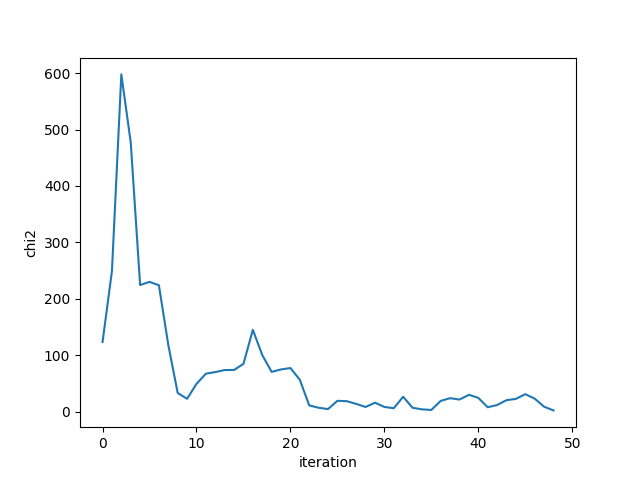
\includegraphics[scale=0.7]{images/doubletetrahedron_02.png}
	\caption{A második dupla tetraéder konvergencia görbéje.}
	\label{fig:doubletetra02}
\end{figure}
%after test chi2 = 9.489499999999996

A \ref{fig:doubletetra02} grafikon az előzővel ellentétben nem mutatott extrém eltéréseket, de sokkal nehezebben tud konvergálni az elvárt értékekhez.
A kapott testen nem olyan látványos az oldallapok közötti különbség mint amire számítottunk.

\newpage

\Section{Oktaéder}

A kezdeti oktaéder csúcsai a középpontjától 50 egység távolságra helyezkednek el, így az oldalélek kicsivel nagyobbak az előzőleg tesztelt testekénél.
A könnyebb inicializálás miatt választottuk a méretének ezen meghatározását.
Az ellenőrzésnél a $\chi^2 < 14.067$ vizsgálatnak kell teljesülnie.

\begin{remark}
A szimulációkban nagyobb hibaküszöböt használunk, mert a test alakja miatt nehezebben közelíthető az eloszlás.
A mintaszámot is növelhetnénk, de akkor a futási idő exponenciálisan nőne.
\end{remark}

Az első testtel a hét érme feldobása során kapott értékek összegét szeretnénk közelíteni.
(Az érmedobás eredményét nullának vagy egynek vesszük.)
A várt binomiális eloszlás: [1/128, 7/128, 21/128, 35/128, 35/128, 21/128, 7/128, 1/128]

\begin{python}
from jelly.py import Octahedron
err = 0.1
N = 1000
threshold = n * err**2
octahedron = Octahedron()
o1 = octahedron.estimateBodyFace2(
     [1/128, 7/128, 21/128, 35/128, 35/128, 21/128, 7/128, 1/128],
     1, threshold, N)[0]
\end{python}

\begin{figure}[h!]
	\centering
	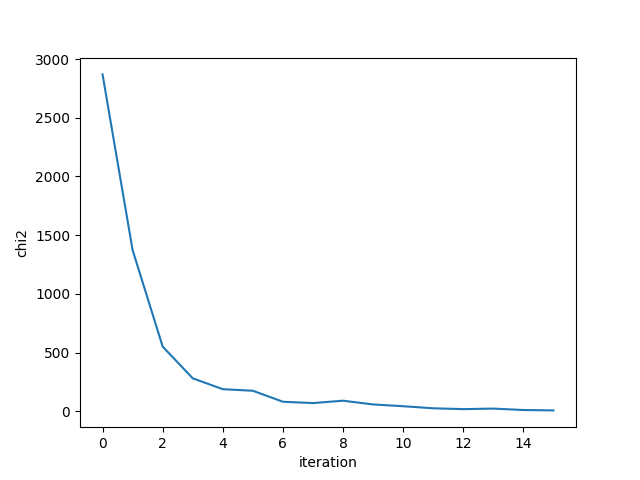
\includegraphics[scale=0.7]{images/octahedron_01.png}
	\caption{Az első oktaéder konvergencia görbéje.}
	\label{fig:octa01}
\end{figure}
%after test chi2 = 65.54
% wrong

A \ref{fig:octa01} grafikonon látható konvergencia alapján ez a legjobb eredmény amit a mérések alatt kaptunk.
ezzel ellentétben az algoritmus leállása után végzett $\chi^2$ próbán nem felelt meg nekünk a test.
Ez annak a következménye, hogy az elvárt eloszlás nehezen közelíthetősége miatt feljebb vittük a hibaküszöböt, és így pontatlanabb mérést kaptunk.
A python kódok lassú futási ideje miatt nem a mintavételt növeltük.

Mivel az egyes valószínűségek rögzítve vannak az oldallapokhoz, így meg tudjuk adni azt, hogy két szemben lévő lapnak nagyobb legyen az előfordulása.
Arra számítunk hogy a kapott testnek az alakja kicsit hasonlítani fog egy hasábra.
A várt eloszlás: [1/4, 1/12, 1/12, 1/12, 1/12, 1/12, 1/12, 1/4]

\begin{python}
from jelly.py import Octahedron
err = 0.1
N = 1000
threshold = n * err**2
octahedron = Octahedron()
o2 = octahedron.estimateBodyFace2(
     [1/4, 1/12, 1/12, 1/12, 1/12, 1/12, 1/12, 1/4],
     1, threshold, N)[0]
\end{python}

\begin{figure}[h!]
	\centering
	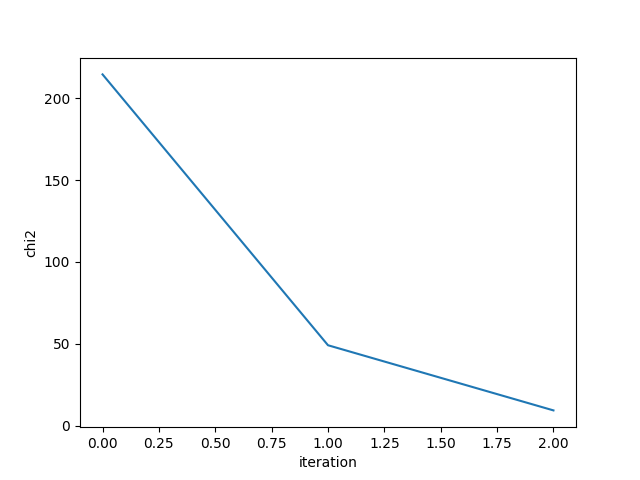
\includegraphics[scale=0.7]{images/octahedron_02.png}
	\caption{A második oktaéder konvergencia görbéje.}
	\label{fig:octa02}
\end{figure}
%after test chi2 = 7.92

description of \ref{fig:octa02}.